\documentclass[a4paper]{article}
\usepackage{graphicx}
\usepackage{wrapfig}

\title{Peptide retention time prediction} 


\author{
Luminita Moruz\\
Science for Life Laboratory,\\
School of Biotechnology,\\
Royal Institute of Technology (KTH),\\
Stockholm, Sweden
\and
Lukas K\"all\\
Science for Life Laboratory,\\
School of Biotechnology,\\
Royal Institute of Technology (KTH),\\
Stockholm, Sweden}


\begin{document}

\maketitle

\setcounter{secnumdepth}{2} % organisational level that receives a numbers
\setcounter{tocdepth}{2}    % print table of contents for level 2
\tableofcontents            % print the table of contents
% levels are: 0 - chapter, 1 - section, 2 - subsection, 3 - subsubsection



\section{Introduction}

Besides decreasing the number of peptides injected at the same time
into the mass spectrometer, the separation process in itself provides
useful information about the analytes. On the one hand, the instrument
always records the time when a peptide elutes from the chromatography
column, i.e. the retention time. On the other hand, the retention time
can also be estimated by examining the sequence of the peptide. The
availability of both predicted and observed retention times has proven
to be a powerful feature, with several applications in mass
spectrometry-based proteomics \cite{Palmblad2013}.  In this chapter,
Sections~\ref{sec:rtpred} and \ref{sec:rtpredm} describe the main
approaches used to estimate retention time from peptide sequences,
while Section~\ref{sec:app} discusses some of the most important
applications of retention time predictions. Section~\ref{sec:irt}
briefly introduces the use of peptide retention standards.


\section{\label{sec:rtpred}Retention time prediction for unmodified peptides}

\begin{wrapfigure}{r}{.45\textwidth}
\vspace{-10pt}
%\begin{figure}[htbp]
\centering
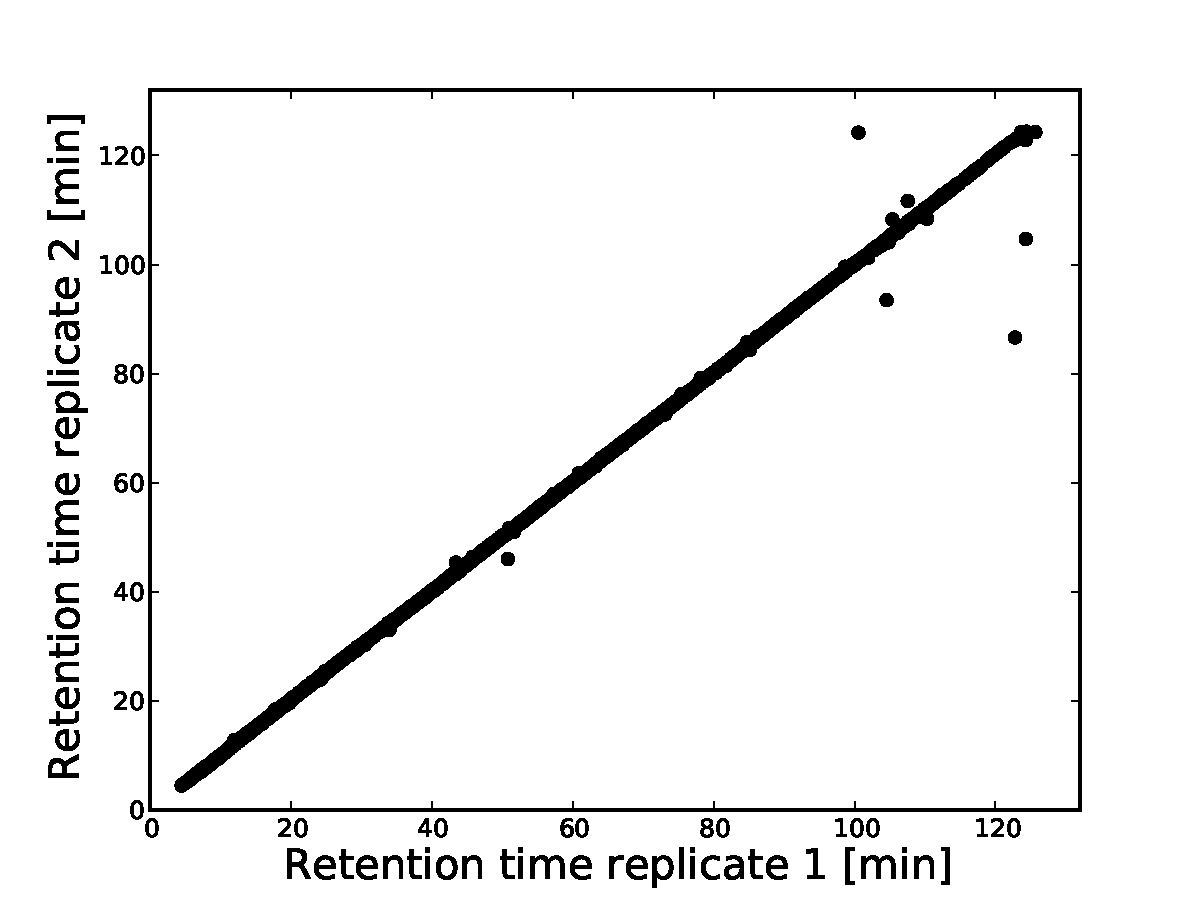
\includegraphics[trim=0.5cm 0cm 2cm 1.5cm, clip=true, width=0.43\textwidth]{img/reproducibility.pdf}
\caption{\label{fig:repr} {\bf Reproducibility of peptide retention time.} Two identical shotgun proteomics experiments were carried out. The retention times of the peptides confidently identified in both runs are displayed.}
%\end{figure}
\vspace{-12pt}
\end{wrapfigure}

Liquid chromatography gives reproducible results. Except for small
shifts from run to run, the same peptide elutes at about the same time
when a sample is reanalyzed under identical experimental conditions
(Figure~\ref{fig:repr}). This suggests that peptides engage in
well-defined interactions during separation, which depend only on the
experimental setup employed and the properties of the peptides
themselves. However, the properties of the peptides are determined to
a large extent by their amino-acid sequence. As a consequence, given a
chromatography setup, the sequence of a peptide should provide
virtually all the information needed to predict its retention time.

\vspace{0.15cm}

Following these observations, a variety of retention time prediction
methods has been proposed. These methods can be roughly divided into
three classes: index-based methods, modeling-based techniques and
machine learning approaches. The main ideas underlying each category
are described below.

\subsection{Index-based methods}
\hyphenation{lear-ning}
\hyphenation{indivi-dual}

% Basic idea 
Index-based prediction methods aim at estimating the effect that each
individual amino acid in a sequence has on the retention time of the
peptide. The individual contributions of the amino acids are often
referred to as retention coefficients, and a set of retention
coefficients forms a retention index. Once a retention index is
derived for a given chromatography system, the retention time of a
peptide can be estimated by simply summing up the retention
coefficients of the constituent amino acids.

\vspace{0.15cm}

% The first method 
The first method to implement this idea used a set of 25 short
peptides together with their observed retention times to derive
retention coefficients for each of the amino acids and end groups
present in the sequences \cite{meek1980}. The coefficients were
calculated using a form of iterative regression and were estimated
using only the amino-acid composition of the peptides, without any
information about the position of each amino acid in the
sequence. However, since shuffled versions of the same peptide
sequence had previously been separated on a RPLC column, the author
pointed out that additional parameters would be required for
predicting the retention time of longer peptides.

%The study reported good correlations between predicted and observed
%retention times, showing that for short peptides the amino acid
%composition provided sufficient information to produce reasonable
%retention time predictions.

\vspace{0.15cm}

% It became available that additional information is needed; anc oclumn is important  examples 
Indeed, a subsequent study showed that even for short peptides,
distinct retention coefficients are obtained when an amino acid is
located at different positions in a sequence \cite{Houghten1987}. In
this context, the authors speculated that different retention
coefficients would be needed for each position in a peptide
sequence. Although the exact chemical mechanisms underlying this
observation are still not fully understood, a number of studies have
pinpointed individual factors that alter the retention coefficients of
amino acids. As an example, it has been shown that the retention
contribution of an amino acid is affected by the overall
hydrophobicity of the peptide \cite{Mant2006}, the number of positive
charges \cite{Mant2006} or presence of elements of secondary
structure \cite{Zhou1990}. In addition, modifications in
chromatography setup such as changing the composition of the mobile or
stationary phases also modify the elution pattern of the
peptides \cite{Browne1982, Guo1987, Gilar2010}.

\vspace{0.15cm}
% SSRcalc was proposed including a number of additional terms; then it was extended
% for a few other column
Following these observations, Krokhin et al. developed
SSRCalc \cite{Krokhin2004}, which is currently the most widely used
index-based retention time predictor. In the initial version of the
algorithm a collection of 346 tryptic peptides was used to derive two
sets of retention coefficients, one corresponding to the N-terminal
and one to all the other positions in a peptide sequence. Furthermore,
correction factors for peptide length and overall hydrophobicity were
included. Subsequent versions of the algorithm included terms
accounting for additional properties such as isoelectric point,
nearest-neighbor effects of charged peptides and propensity to form
helical structures \cite{Krokhin2006}. However, a limitation of the
approach is that the algorithm was optimized for predicting retention
times for certain chromatography setups. Thus, SSRCalc's prediction
ability deteriorates for experimental conditions diverging from the
setup on which the algorithm was optimized \cite{Spicer2007}.

% - sum of retention coefficients (Meek reference 22) - different RT
% coefficients and the observation that this coefficients depend on
% the chromatography system (Browne ref 24) - investogate the
% contribution of individual amino acids (Guo 26,27) - all the work
% above was done on synthetic peptides os simple samples. Then RT
% prediction for complex sa% mples was proposed by (Palmblad 28-30) -
% important the exact position of each aa (pref 27) - additional rules
% included peptide length (ref 32), position of K and R residues [ref
% 33], and in the e% nd that the position of each amino acid at each
% position is important [ref 34] - amphipathicity [ref 35] - SSRCalc
% [ref 36-39]


\subsection{Modeling-based approaches}

Modeling-based techniques predict retention times by using information
about the structure of the peptides and/or their chemical interactions
during separation. An example is the methods based on Quantitative
Structure-Retention Relationships (QSRR) \cite{Kaliszan2005,
Baczek2005}. In such approaches specialized molecular modeling
software is used to calculate a number of chemical descriptors from
the peptide sequence. The most relevant such descriptors are then
selected and combined via regression analysis into a prediction
function, which is subsequently used to estimate retention time for
other peptides of interest.

\vspace{0.15cm}

In other modeling-based approaches theoretical models are used to
capture the chemical behavior of peptides on the chromatography
column. One such method is BioLCCC, which attempts to model the
connectivity of the amino acids in a peptide chain and the general
mechanisms of chromatographic
separation \cite{gorshkov2006}. Nevertheless, given the numerous
factors involved in peptide separation, modeling approaches often
involve a considerable number of simplifications.

 
\subsection{Machine learning-based methods}

In machine learning-based approaches a set of training peptides,
i.e. peptide sequences with known retention times, are used to
customize a predefined mathematical model. This step is typically
called training or learning. Once trained, the mathematical model can
be subsequently used to predict retention time for other peptides of
interest.

\vspace{0.15cm}

One of the first machine learning approaches for retention time
prediction was based on an Artificial Neural Network
(ANN) \cite{petritis2003}. Initially, each peptide was described by 20
features giving the number of each of the 20 amino acid residues
present in the sequence. The network was trained using $\sim$7000
peptides with known retention times and evaluated using a set of
$\sim$5000 peptides originating from another organism. The algorithm
reported good accuracies, especially taking into account that it only
used information about the amino acid composition of the peptides.

\vspace{0.15cm}

In a follow-up work, the method was extended by representing each
 peptide by 1052 instead of 20
 features \cite{petritis2006improved}. The new descriptors encoded the
 identity of each amino acid at each position in a sequence, as well
 as the length and the hydrophobic moment of the peptide. The new
 neural network was trained on more than 300,000 peptide sequences. To
 obtain such a large number of peptides with known retention times, a
 strategy to normalize elution times was developed. This allowed
 pooling of peptides identified in more than 12,000 shotgun
 experiments. The trained algorithm reported excellent performance for
 the 1303 peptides on which it was evaluated.

\vspace{0.15cm}

A drawback of the method was however the large amount of training
peptides required, which made the algorithm difficult to retrain for
other chromatographic conditions. This was a serious limitation in the
context of RPLC separation, where a broad variety of chromatographic
setups is commonly used across research laboratories. To address this,
Klammer et al. proposed a predictor based on support vector machines
(SVMs) \cite{klammer2007improving}. Their method required fewer
training peptides and could thus be easily adapted to new
chromatographic conditions, but yielded lower prediction
accuracies. Subsequently, a more elaborate SVM-based method using a
customized kernel function was proposed \cite{rtpredictImproved}. This
approach provided reasonable prediction accuracy, while requiring as
little as 50 peptides for training.

% Other retention time prediction method used a feature selection
% approach to select relevant descriptors, and showed good
% performances even for longer peptides containing up to 50 amino
% acids \cite{shinoda2006}.

\vspace{0.15cm}

However, despite all these efforts, it should be pointed out that none
of the retention time prediction methods currently available is able
to provide accuracies comparable to the small shifts observed when
running a sample twice through a chromatography column
(Figure \ref{fig:repr}). Recently, the lack of suitable
representations for secondary structure elements was indicated as one
of the main causes of prediction errors \cite{Reimer2012}.  Most
probably additional factors are involved, and further endeavors are
required to reach the desired level of accuracy.


\section{\label{sec:rtpredm}Retention time prediction for modified peptides}

% very few studies have documented the chromatographic behavior of
% modified peptides
The study of peptide separation mechanisms in RPLC has been an active
area of research for the past 30 years. Nonetheless, surprisingly
little efforts have been directed toward investigating the
chromatographic behavior of posttranslationally modified peptides. The
few studies available so far have mostly focused on phosphorylated
peptides \cite{Kim2007}, or a couple of artifactual modifications
commonly introduced during sample
preparation \cite{Reimer2011}. Consequently, few retention time
prediction methods have been extended and assessed for such
peptides. A majority of the approaches currently available are
modification-specific, many of them developed specifically for
phosphopeptides \cite{Kawakami2005, perlova2010}.

\vspace{0.15cm}

As large-scale studies of a variety of posttranslational modifications
increasingly come within reach (Section \ref{sec:ptms}), predictors
handling other modifications will become available. In this context,
machine learning methods are expected to play an important role
because of their flexibility and intrinsic ability to adapt to new
datasets.


\section{\label{sec:app}Applications of retention time prediction}

% RT prediction is used to increase number of identifications 
The time points when peptides elute from the RPLC column are typically
recorded in MS experiments. By comparing these values with predicted
retention times for peptides from a sequence database, information
about the identity of the peptides can be obtained. This relatively
straightforward idea has been implemented in a variety of flavors and
was proven to bring significant improvements in the peptide
identification process.

\vspace{0.15cm}

Palmblad et al. showed that matching theoretical and observed masses
and retention times provides a simple, yet powerful method to identify
peptides in simple biological
mixtures \cite{palmblad2002prediction}. Strittmatter et al. used
retention time as a parameter in a discriminant function that
differentiated between correct and incorrect peptide
identifications \cite{Strittmatter2004}. Following this approach, they
reported $\sim$9\% more confident peptide identifications in a typical
shotgun experiment. Along the same lines, Klammer et al. demonstrated
that for specific experimental conditions, just filtering out peptides
with large deviations between observed and predicted retention time
leads to up to 50\% more
identifications \cite{klammer2007improving}. 

\vspace{0.15cm}

Krokhin et al. illustrated yet another route to employ retention time
predictions \cite{krokhin200612, McQueen2012}. They showed that
theoretical retention times and mass measurements can be used to
define lists of peptides belonging to already identified proteins. The
instrument can be instructed to avoid fragmenting these peptides, thus
decreasing the number of fragmentation events that need to be acquired
for identifying a set of proteins.

\vspace{0.15cm}

% Improve the design of SRM experiments 
In addition, predicted retention times can also be used to investigate
the elution properties of the peptides, and possibly design improved
experimental setups. As an example, Bertsch et al. employed retention
time predictions to design {\em de novo} targeted proteomic
assays \cite{bertsch2010}. Other applications include decreasing the
number of candidate peptides during database
searching \cite{lobas2013} and simulations of MS-based
experiments \cite{bielow2011}.


% It is an orthogonal information. Decrease the database search space,
% study properties of the peptides
 
\section{\label{sec:irt}Peptide retention standards}

\hyphenation{wide-spread}
% peptide standards what they are, what they are used for 
In the past years, the use of retention standards has become
increasingly widespread in the context of mass spectrometry-based
proteomics~\cite{olegstd, irt}. Such standards typically consist of a
small number of peptides covering a wide span of hydrophobicities and
with well studied behaviors under LC-MS/MS. These peptides are often
analyzed together with the sample of interest, and by comparing their
observed and expected behaviors one can obtain valuable information
for a variety of applications.

\vspace{0.15cm}

As an example, in targeted proteomics peptide standards can be used to
 calibrate predicted retention times and to estimate the accuracy of
 the prediction algorithms~\cite{Kiyonami01022011}. In addition,
 recent studies have reported excellent results when using peptide
 standards to adjust the time when certain transitions are scheduled
 ``on-the-fly''~\cite{seb, irt}. Retention standards are also useful
 for aligning data from multiple experiments~\cite{petritis2003}, to
 transfer retention times between different chromatography
 setups~\cite{seb}, or to keep track of the performance of LC-MS/MS
 systems~\cite{qcal}.

\bibliographystyle{unsrt}
\bibliography{./retention.bib}


\end{document}
